\documentclass[compress]{beamer}
\usetheme{sthlm}

%-=-=-=-=-=-=-=-=-=-=-=-=-=-=-=-=-=-=-=-=-=-=-=-=
%        LOADING BEAMER PACKAGES
%-=-=-=-=-=-=-=-=-=-=-=-=-=-=-=-=-=-=-=-=-=-=-=-=

\usepackage{
booktabs,
datetime,
dtk-logos,
graphicx,
multicol,
pgfplots,
ragged2e,
tabularx,
tikz,
wasysym,
multirow,
float,
caption,
subcaption
}

\pgfplotsset{compat=1.8}

\usepackage[utf8]{inputenc}
\usepackage[portuguese]{babel}
\usepackage[T1]{fontenc}
\usepackage{newpxtext,newpxmath}
\usepackage{listings}

\lstset{ %
language=[LaTeX]TeX,
basicstyle=\normalsize\ttfamily,
keywordstyle=,
numbers=left,
numberstyle=\tiny\ttfamily,
stepnumber=1,
showspaces=false,
showstringspaces=false,
showtabs=false,
breaklines=true,
frame=tb,
framerule=0.5pt,
tabsize=4,
framexleftmargin=0.5em,
framexrightmargin=0.5em,
xleftmargin=0.5em,
xrightmargin=0.5em
}



%-=-=-=-=-=-=-=-=-=-=-=-=-=-=-=-=-=-=-=-=-=-=-=-=
%        LOADING TIKZ LIBRARIES
%-=-=-=-=-=-=-=-=-=-=-=-=-=-=-=-=-=-=-=-=-=-=-=-=

\usetikzlibrary{
backgrounds,
mindmap
}

%-=-=-=-=-=-=-=-=-=-=-=-=-=-=-=-=-=-=-=-=-=-=-=-=
%        BEAMER OPTIONS
%-=-=-=-=-=-=-=-=-=-=-=-=-=-=-=-=-=-=-=-=-=-=-=-=

\setbeameroption{show notes}

%-=-=-=-=-=-=-=-=-=-=-=-=-=-=-=-=-=-=-=-=-=-=-=-=
%        BEAMER COMMANDS
%-=-=-=-=-=-=-=-=-=-=-=-=-=-=-=-=-=-=-=-=-=-=-=-=


%-=-=-=-=-=-=-=-=-=-=-=-=-=-=-=-=-=-=-=-=-=-=-=-=
%
%	PRESENTATION INFORMATION
%
%-=-=-=-=-=-=-=-=-=-=-=-=-=-=-=-=-=-=-=-=-=-=-=-=

\title{Processos}
\subtitle{DCE540 - Computação Paralela e Distribuída}
%\date{\small{\jobname}}
\author{\texttt{Iago Carvalho}}
\institute{\texttt{Departamento de Ciência da Computação}}

\hypersetup{
pdfauthor = {Iago A. Carvalho},      
pdfsubject = {Computação Paralela e Distribuída},
pdfkeywords = {},  
pdfmoddate= {D:\pdfdate},          
pdfcreator = {WriteLaTeX}
}

\begin{document}

\begin{frame}
\titlepage

\end{frame}

%% --------------------------------------------------------

\begin{frame}{Processos}

A definição de \textbf{processo} vem da área de sistemas operacionais
\begin{itemize}
    \item Um programa em execução
    \item Gerenciar processos é uma das tarefas mais importantes de um sistema operacional
\end{itemize}

\vspace{0.5cm}

A definição de processo no conceito de computação paralela e distribuída é um pouco diferente
\begin{itemize}
    \item Threads
    \item Multi-core
    \item Multi-processadores
    \item Virtualização
\end{itemize}

% \begin{columns} % align columns
% \begin{column}{.48\textwidth}

% Devido a estas características e a falta de boas maneiras de conectar um PC a outro, cada máquina operava tradicionalmente isolada das outras.

% \end{column}%
% \hfill%
% \begin{column}{.48\textwidth}


% 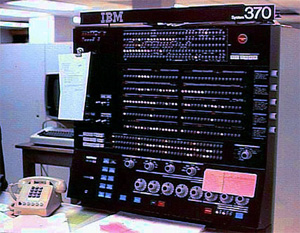
\includegraphics[width=0.85\textwidth]{images/ibm_370.jpg}
% \end{column}%
% \end{columns}

\end{frame}

%% --------------------------------------------------------

\begin{frame}{Processos em sistemas distribuídos}

Em um sistema distribuído, um processo não pertence exclusivamente a um sistema operacional
\begin{itemize}
    \item Um processo pode ser movido de um nó para outro
    \begin{itemize}
        \item Escalabilidade
        \item Tolerância a falhas
        \item Balanceamento de carga
    \end{itemize}
\end{itemize}

\vspace{0.5cm}

Para falarmos de processos, primeiramente devemos apresentar o conceito de \textbf{threads}
\begin{itemize}
    \item Um processo em um sistema distribuído pode ser dividido em múltiplas threads
\end{itemize}
\end{frame}

%% --------------------------------------------------------

\begin{frame}{Threads}

Threads também são chamadas de \textit{processos leves}
\begin{itemize}
    \item Sistema operacional faz o gerenciamento de threads de forma mais simples e rápida
    \item Seu contexto é muito menor do que o de um processo
    \item Menor segurança
    \begin{itemize}
        \item Segurança é de responsabilidade do desenvolvedor/programador
    \end{itemize}
\end{itemize}

\vspace{0.5cm}

Existe um grande número de outras diferenças entre processos e threads, como a seguir

\end{frame}

%% --------------------------------------------------------

\begin{frame}{Processo \textit{vs} thread}

\begin{table}[]
\centering
\resizebox{\textwidth}{!}{%
\begin{tabular}{@{}cc@{}}
\toprule
\textbf{Processo}                              & \textbf{Thread}                                     \\ \midrule
Processo pesado                       & Processo leve                              \\ \midrule
\multirow{2}{*}{\begin{tabular}[c]{@{}c@{}}Depende do sistema operacional para\\ realizar troca entre processos\end{tabular}} &
  \multirow{2}{*}{\begin{tabular}[c]{@{}c@{}}Independente do sistema operacional para\\ realizar troca entre threads\end{tabular}} \\
                                      &                                            \\ \midrule
Processos são independentes           & Uma thread pode alterar outras             \\ \midrule
Possui memória e arquivos próprios    & Compartilham memória e arquivos            \\ \midrule
Pesado para ser criado                & Leve para ser criado                       \\ \midrule
Criação depende de chamada de sistema & Criação independente de chamada de sistema \\ \midrule
Utiliza grande quantidade de recursos & Utiliza uma menor quantidade de recursos   \\ \midrule
\multirow{2}{*}{\begin{tabular}[c]{@{}c@{}}Se um processo é bloqueado, os processos\\ relacionados também são\end{tabular}} &
  \multirow{2}{*}{\begin{tabular}[c]{@{}c@{}}Se uma thread é bloqueada, outras threads \\ relacionadas ainda estão livres\end{tabular}} \\
                                      &                                            \\ \bottomrule
\end{tabular}%
}
\end{table}

\end{frame}

%% --------------------------------------------------------

\begin{frame}{Processo mono \textit{vs}  multi-thread}

\vspace{1cm}

\centering 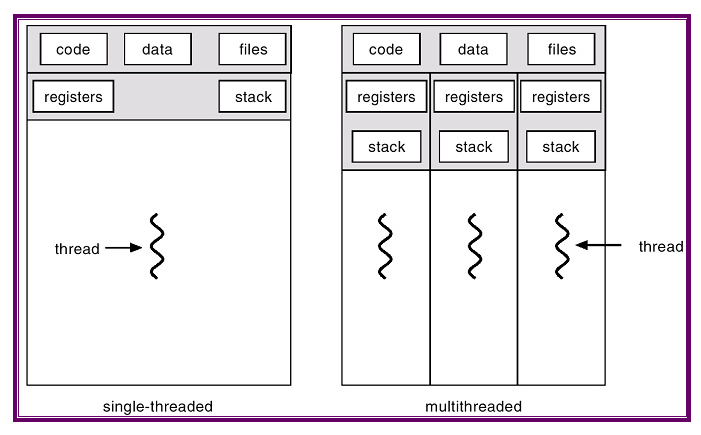
\includegraphics[width=\textwidth]{images/multi-thread.png}
\end{frame}

%% --------------------------------------------------------

\begin{frame}{Threads em sistemas distribuídos}

Uma das propriedades mais importantes de threads em sistemas distribuídos é sua capacidade de ser bloqueada sem que o processo inteiro seja também bloqueado
\begin{itemize}
    \item Maneira simples de implementar comunicação assíncrona
\end{itemize}

\vspace{0.5cm}

Outra aplicação de threads é no desenvolvimento de servidores
\begin{itemize}
    \item Servidores podem receber um grande número de requisições
    \item Cada requisição cria uma thread
    \begin{itemize}
        \item Requisições são tratadas de forma paralela
    \end{itemize}
\end{itemize}
\end{frame}

%% --------------------------------------------------------

\begin{frame}{Servidor multi-thread}

\vspace{1cm}

\centering 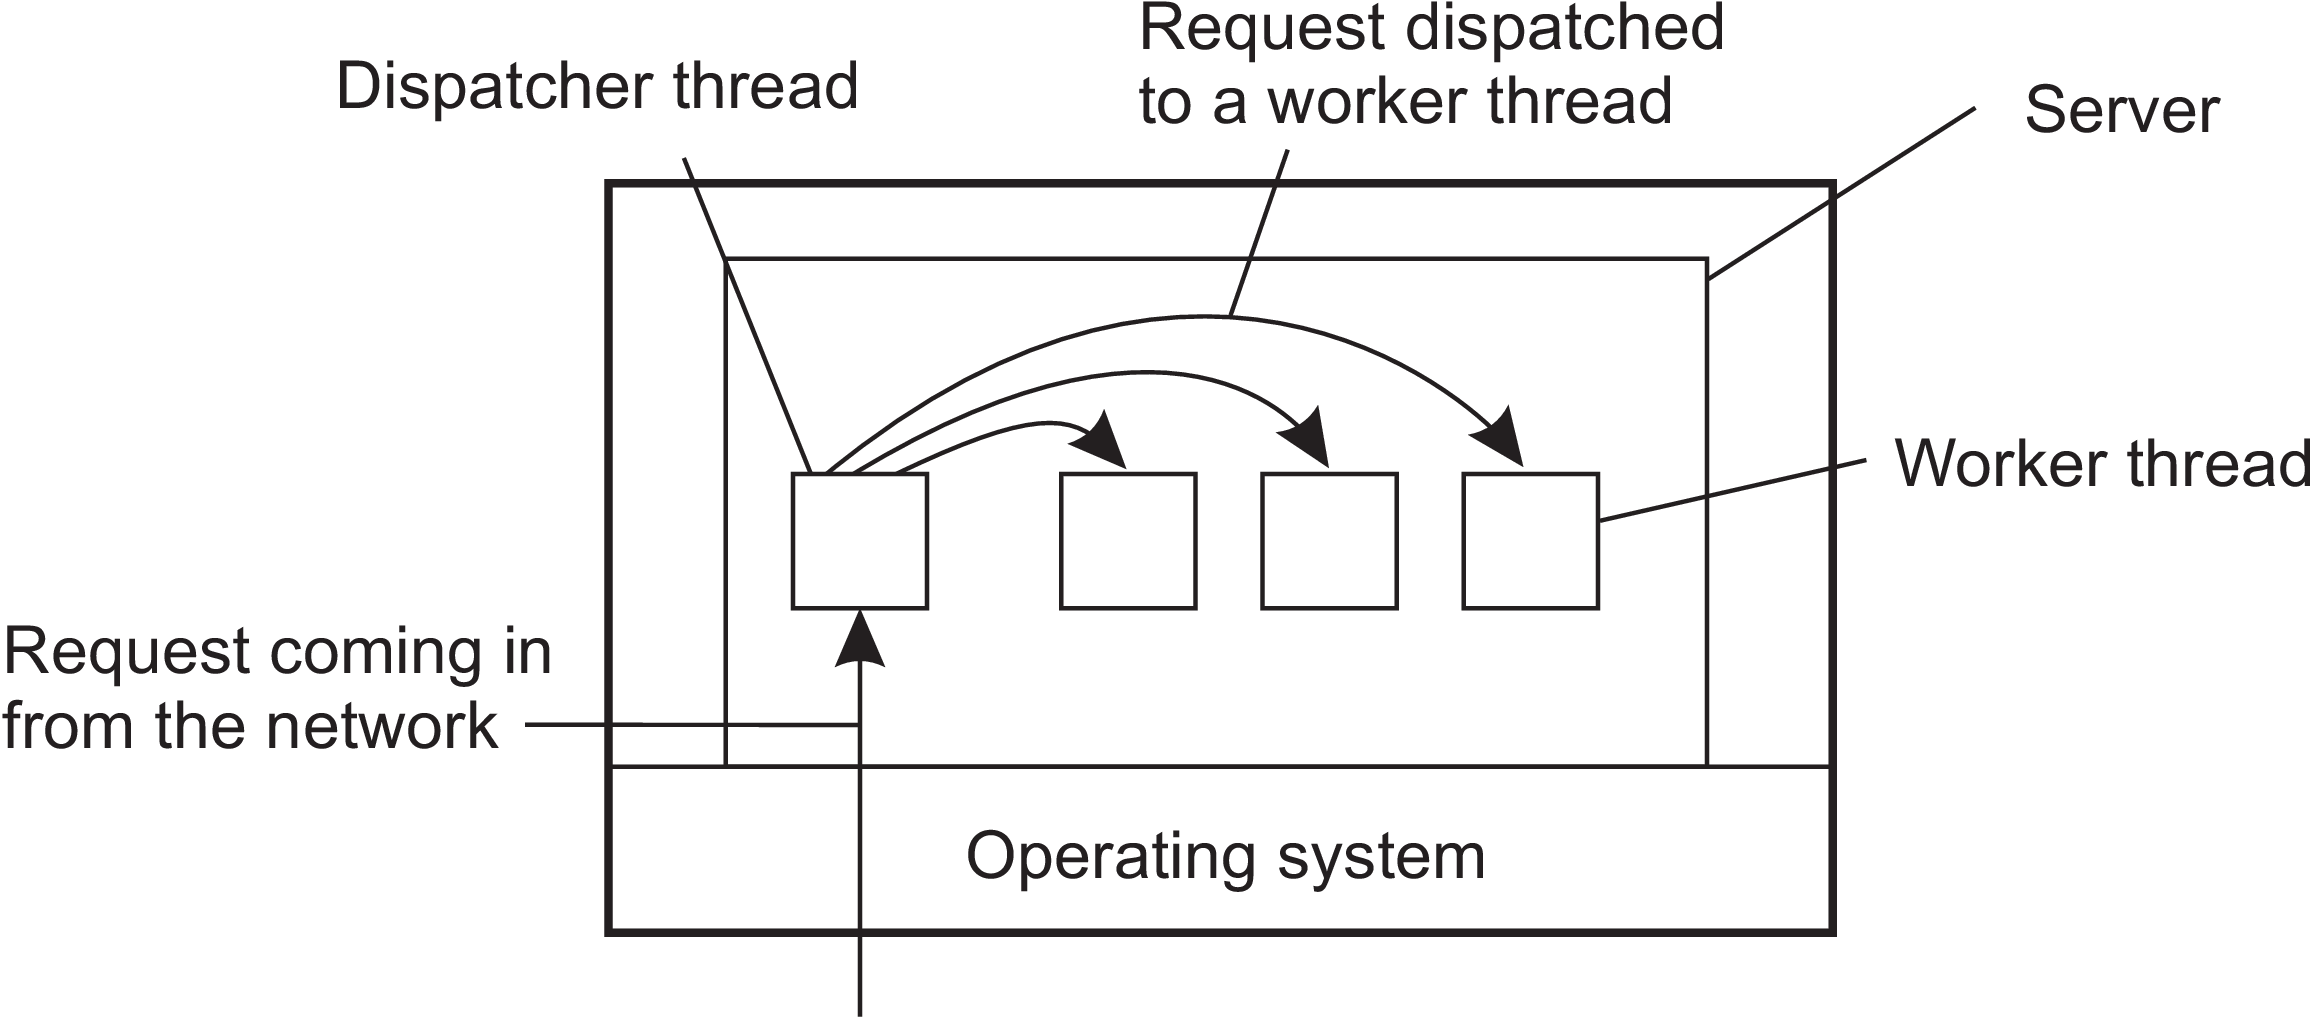
\includegraphics[width=\textwidth]{images/servidor_threads.png}
\end{frame}

%% --------------------------------------------------------

\begin{frame}{Clientes multi-thread}

Além de servidores, também é interessante que clientes sejam implementados utilizando o conceito de multi-thread
\begin{itemize}
    \item Realizar comunicação assíncrona
    \item Utiliza a natureza não-blocante das threads
\end{itemize}

\vspace{0.5cm}

Exemplo de aplicação: navegador \textit{web}

\end{frame}

%% --------------------------------------------------------

\begin{frame}{Navegadores \textit{web}: gerenciamento de janelas}

\centering 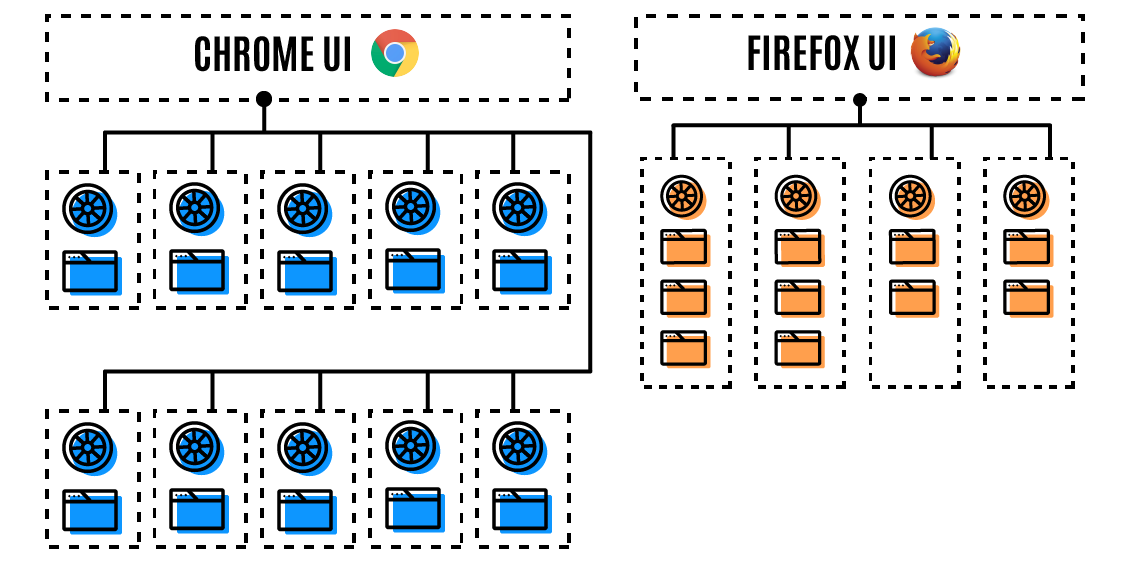
\includegraphics[width=\textwidth]{images/browser_example1.png}

\end{frame}

%% --------------------------------------------------------

\begin{frame}{Navegadores web: requisições assíncronas}

\centering 
\includegraphics[width=0.7\textwidth]{images/browser_example2.png}

\end{frame}

%% --------------------------------------------------------

\begin{frame}{Virtualização}

A ideia de utilizar diversas threads é executar múltiplas tarefas em paralelo.

\vspace{0.5cm}

Entretanto, em um único processador, somente uma única instrução (ou algumas, em casos de pipeline) pode ser relizada por clock
\begin{itemize}
    \item É criado a ilusão de paralelismo através da troca extremamente rápida entre threads (ou processos)
\end{itemize}

\vspace{0.5cm}

A essa ilusão de processamento paralelo, nós damos o nome de \textit{virtualização} de recursos
\end{frame}

%% --------------------------------------------------------

\begin{frame}{Virtualização em processadores}

\centering 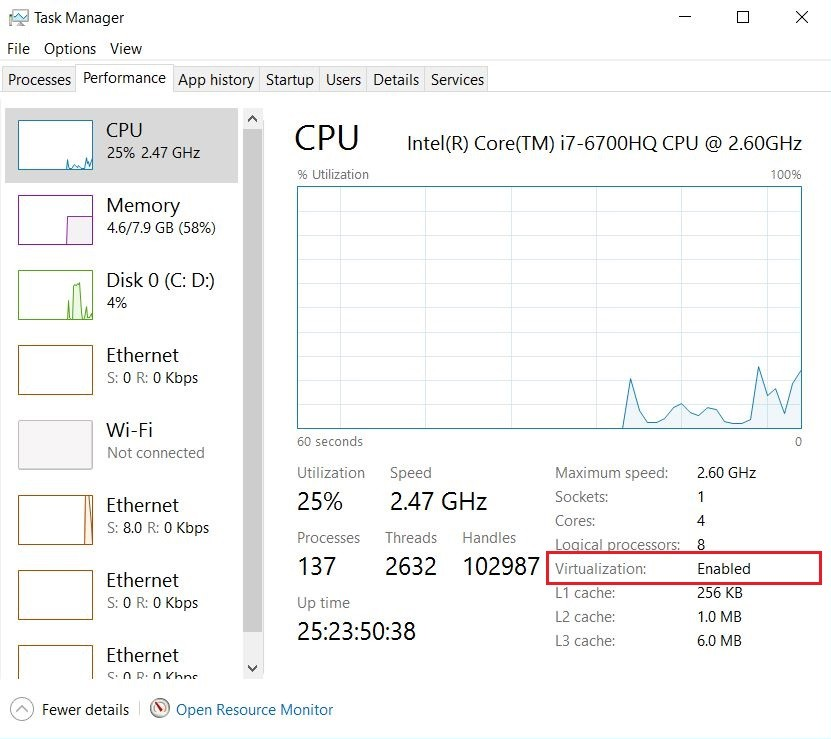
\includegraphics[width=0.7\textwidth]{images/task_manager.png}

\end{frame}

%% --------------------------------------------------------

\begin{frame}{Usos de virtualização}

Além disso, existem três usos adicionais de virtualização em sistemas distribuídos


Infrastructure-as-a-Service (IaaS)
\begin{itemize}
    \item Serviços de nuvem, como processamento e armazenamento de dados
\end{itemize}

Platform-as-a-Service (PaaS)
\begin{itemize}
    \item IaaS + plataformas de software 
\end{itemize}

Software-as-a-Service (SaaS)
\begin{itemize}
    \item PaaS + aplicações
\end{itemize}

\end{frame}

%% --------------------------------------------------------

\begin{frame}{Virtualização em sistemas distribuídos}

\centering 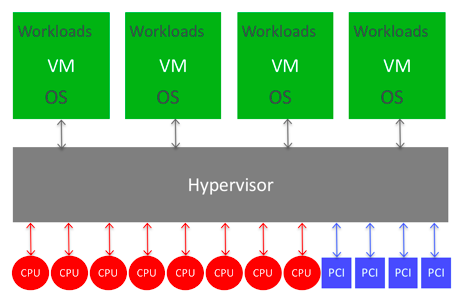
\includegraphics[width=\textwidth]{images/iaas.png}

\end{frame}

%% --------------------------------------------------------

\begin{frame}{Pizza?}

\centering 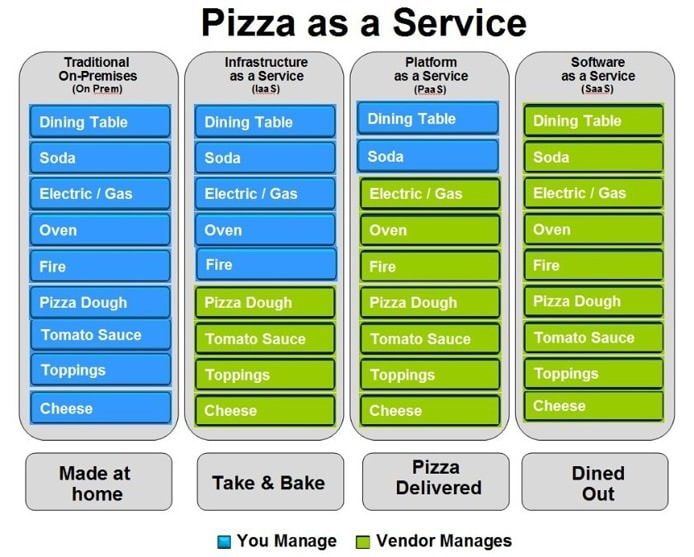
\includegraphics[width=\textwidth]{images/virtualizacao_pizza.jpg}

\end{frame}

%% --------------------------------------------------------

\begin{frame}{Computadores!}

\centering 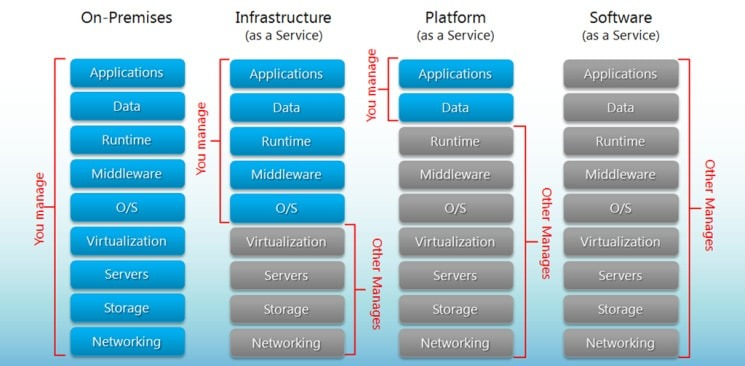
\includegraphics[width=\textwidth]{images/virtualizacao_comparacao.jpg}

\end{frame}

\end{document}